%%%%%%%%%%%%%%%%%%%%%%%%%%%%%%%%%%%%%%%%%
% FRI Data Science_report LaTeX Template
% Version 1.0 (28/1/2020)
% Jure Demšar (jure.demsar@fri.uni-lj.si)
%
% Based on MicromouseSymp article template by:
% Mathias Legrand (legrand.mathias@gmail.com)
% With extensive modifications by:
% Antonio Valente (antonio.luis.valente@gmail.com)
%
% License:
% CC BY-NC-SA 3.0 (http://creativecommons.org/licenses/by-nc-sa/3.0/)
%
%%%%%%%%%%%%%%%%%%%%%%%%%%%%%%%%%%%%%%%%%


%----------------------------------------------------------------------------------------
%	PACKAGES AND OTHER DOCUMENT CONFIGURATIONS
%----------------------------------------------------------------------------------------
\documentclass[fleqn,moreauthors,10pt]{ds_report}
\usepackage[english]{babel}

\graphicspath{{fig/}}

\usepackage{graphicx}
\usepackage{caption}
\captionsetup{justification=justified}

\usepackage{placeins}

%----------------------------------------------------------------------------------------
%	ARTICLE INFORMATION
%----------------------------------------------------------------------------------------

% Header
\JournalInfo{UL FRI Machine Learning for Data Science, 2023-2024}

% Interim or final report
%\Archive{Interim report}
\Archive{Project 1 Report}

\PaperTitle{Random Forest implementation and evaluation} % Article title

% Authors and their info
\Authors{Aljaž Konec\textsuperscript{1}}
\affiliation{\textsuperscript{1}\textit{ak3883@student.uni-lj.si}}

% Multiple authors
%\Authors{John Doe\textsuperscript{1}, Jane Doe\textsuperscript{2}, and Mike Smith\textsuperscript{3}}
%\affiliation{\textsuperscript{1}\textit{john.doe@fri.uni-lj.si}}
%\affiliation{\textsuperscript{1}\textit{jane.doe@fri.uni-lj.si}}
%\affiliation{\textsuperscript{1}\textit{mike.smith@fri.uni-lj.si}}

% Keywords
\Keywords{}
\newcommand{\keywordname}{Keywords}


%----------------------------------------------------------------------------------------
%	ABSTRACT
%----------------------------------------------------------------------------------------

\Abstract{
In this report we present our implementation of the Random Forest classification model and evaluate its performance on the provided FTIR dataset. 
We show that the Random Forest model produces a missclassification rate of 5.1 $\pm$ 2.9\% on the test set, which is significantly lower than using a single full tree with missclassification rates of 17.2 $\pm$ 4.95\%.
This shows that the Random Forest model is more stable and has a lower missclassification rate and can be used as a good baseline for further model development.
}
%----------------------------------------------------------------------------------------

\begin{document}

% Makes all text pages the same height
\flushbottom

% Print the title and abstract box
\maketitle

% Removes page numbering from the first page
\thispagestyle{empty}

%----------------------------------------------------------------------------------------
%	ARTICLE CONTENTS
%----------------------------------------------------------------------------------------

\section*{Introduction}

Random Forests are a popular and powerful machine learning algorithm that can be used for both classification and regression tasks.
They provide a good baseline for many problems and are often used as a benchmark for other machine learning models.
First, we present our implementation of the Random Forest algorithm, then we evaluate the performance on the provided FTIR dataset.


%----------------------------------------------------------------------------------------


\section*{Implementation}

Random Forests are an ensemble learning method that operate by constructing a multitude of decision trees at training time and outputting the majority class of the individual trees for classification tasks or the mean prediction for regression tasks.
In this report we focus only on classification tasks and as such we implement classification trees.

\subsection*{Decision Trees}
Trees are constructed using a greedy algorithm that selects the best split at each tree node.
This splits the data into two subsets and the process is repeated until a stopping criterion is met.
In our implementation we use the Gini impurity to select the best split.
The Gini impurity is a measure of how often a randomly chosen element from the set would be incorrectly labeled if it was randomly labeled according to the distribution of labels in the subset.
It is given by the following formula:
\begin{equation}
	G = 1 - \sum_{i=1}^{n} p_i^2
\end{equation}
Where $p_i$ is the probability of class $i$ in the dataset.
To find the best split at tree node $t$ we first calculate the current Gini impurity $G_{current}$ on the whole dataset $D$.
Then for each feature $f$ and each unique value $v$ of that feature we calculate the Gini impurity $G_{split}$ as the weighted average of the Gini impurities of the two subsets $D_{left}$ and $D_{right}$:
\begin{equation}
	G_{split}(f, v) = \frac{|D_{left}(f, v)|}{|D|} G_{left} + \frac{|D_{right}(f,v)|}{|D|} G_{right}
\end{equation}
Where $D_{left}(f, v)$ is the dataset of all samples where feature $f$ has value less than $v$, dataset $D_{right}(f, v)$ has all samples where feature $f$ has value greater or equal to $v$ and $G_{left}$ and $G_{right}$ are the Gini impurities of the two subsets.

The best split is then the one that maximizes Gini gain 
\begin{equation}
	G_{gain} = G_{current} - G_{split}
\end{equation}

After the best split is found, the process is repeated for the two subsets until a stopping criterion is met.
In our implementation the stopping criterion is:
\begin{enumerate}
	\itemsep-1mm 
	\item Number of samples is less then 2
	\item Gini impurity is 0, which means all samples in the node belong to the same class
\end{enumerate}

\subsection*{Random Forest}
As stated before, Random Forests are a collection of $n$ trees that return the majority class of the individual trees.
This helps to reduce overfitting and increase the generalization of the model since trees are show to overfit substantially to the training data.
To reduce overfitting we use two methods:

\textbf{1. Bagging} is a method that takes the original dataset and creates $n$ new datasets $\{X_i\}_{i=1}^n$ by sampling with replacement.
Each of these new datasets is then used to train a new tree.
This helps to reduce the variance of the model as well as reduce overfitting.

\textbf{2. Feature subsampling} is used to further reduce correlation between trees.
This is done by selecting a random subset of features at each split.
In our implementation we use $\sqrt{p}$ features where $p$ is the total number of features in the dataset.

After all trees are built, the model returns the majority class of the individual trees as the final prediction.
For each tree in the forest we also store the out of bag (OOB) samples as we will use them as evaluation dataset of variable importance in the next section.

%----------------------------------------------------------------------------------------

\section*{Evaluation}
The FTIR dataset consists of 188 samples and 198 features.
For training we used the first 130 samples and for testing the remaining 58 samples.
We trained the Random Forest model with 100 trees and evaluated missclassification rates on the test set.
The OOB samples for each tree were individually used to calculate variable importance.

\subsection*{Misclassification rates}
Missclassification rates on the training dataset are not shown as they are 0\% for both models.
This is expected as we build full trees that perfectly fit the training data and in the case of Random Forest, despite ussing Bagging each of the training samples appears in multiple trees which marks the majority class as the correct one. 
The missclassification rates on the test set are shown in Table \ref{tab:missclassification}.
\begin{table}[!ht]
	\centering
	\begin{tabular}{|l|l|}\hline
        Model & Missclasfication (\%) \\ \hline
        Full Tree & 17.2 $\pm$ 4.95 \\ \hline
        Random Forrest & 5.1 $\pm$ 2.9 \\ \hline
    \end{tabular}
	\caption{Missclassification rates on the test set.}
    \label{tab:missclassification}
\end{table}
The Random forest model has a significantly lower missclassification rate than the full tree model.
The uncertainty of the missclassification rate is also lower for the Random Forest model, indicating that the model is more stable.
Uncertainty was calculated as the standard deviation of the missclassification rates devided by the square root of the number of samples.

\begin{figure}[!ht]
	\centering
	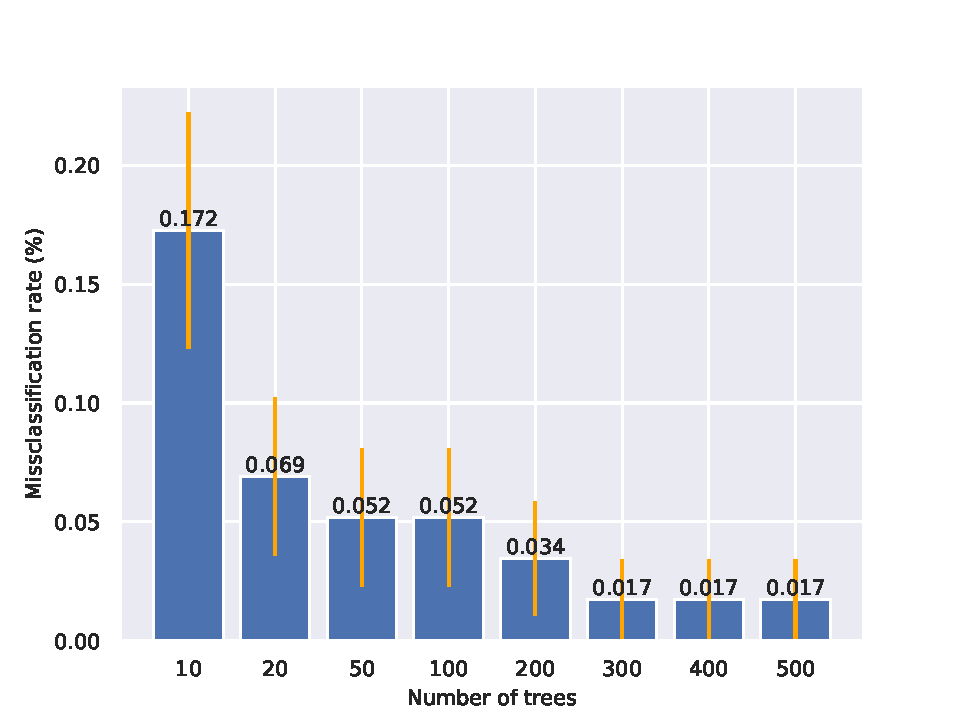
\includegraphics[width=0.5\textwidth]{missclassification.pdf}
	\caption{Missclassification rate of the Random Forest model with different number of trees.}
	\label{fig:missN}
\end{figure}
To further evaluate missclassification of the Random Forest model, Figure \ref{fig:missN} shows how the missclassification rate changes with the number of trees in the forest.
It can be seen that after 200 trees the missclassification rate does not change significantly, indicating that the model has converged.
An argument can be made that 50 trees would be enough for this dataset as the missclassification rate does not change significantly after that.

\subsection*{Variable importance}
Variable importance is calculated using the OOB samples for each corresponding tree in the forest.
This is done by randomly permuting the values of each feature and calculating the change in missclassification rate.
Then, the importance of each feature is calculated as the average change in missclassification rate over all trees.
The variable importance for the 10 most important features is shown in Figure \ref{fig:importance}.
\begin{figure}[!ht]
	\centering
	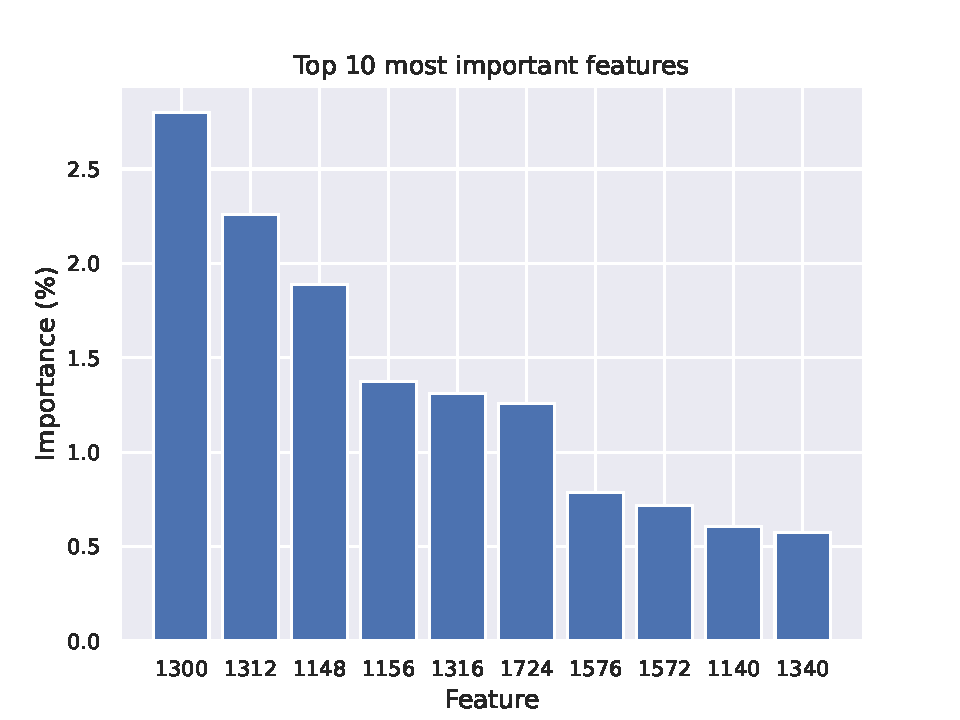
\includegraphics[width=0.5\textwidth]{importance.pdf}
	\caption{Variable importance of the Random Forest model.}
	\label{fig:importance}
\end{figure}
It can be seen that the first 3 features represent a 2\% change in missclassification rate, the next 3 features represent a 1\% change and the last 4 features represent a 0.5\% change.
This implies that the target variable is not strongly dependent on any single feature, but rather on a combination of features.


%----------------------------------------------------------------------------------------

\section*{Conclusion}
Random Forests are a powerful machine learning algorithm that can be used for both classification and regression tasks.
In the FTIR dataset we showed that the Random Forest model has a significantly lower missclassification rate than the full tree model and that the model is more stable.
We have also shown that the random forrest produces a very high accuracy rate which gives a good baseline for developing further models.

%------------------------------------------------

\end{document}
